\testCom
{%Номер задачи
	3.15
}
{%Условие
	Найти период малых поперечных колебаний шарика массы $m$ = 40г, укреплёного на середине натянутой струны длины $l$ = 1 м. Силу натяжения струны считать постоянной и равной $F$ = 10 Н. Массой струны и силами тяжести пренебречь.
}
{%Дано
	дано
}
{%Найти
	$T$
}
{%Решение
	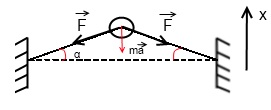
\includegraphics[height=30mm]{3_15.jpg}\\
	$m \frac{d^2x}{dt^2} = - 2 F \sin \alpha$\\
	$\sin \alpha \approx \tg \alpha \approx \frac{2x}{l}$\\
	$m\frac{d^2x}{dt^2} \approx - 2 F \frac{2x}{l}$\\
	$\frac{d^2x}{dt^2} \approx - \frac{4 F}{m l}x = - \omega^2 x\Rightarrow \omega = 2 \sqrt{\frac{F}{ml}}$\\
	$T = \frac{2\pi}{\omega}=\pi \sqrt{\frac{ml}{F}}$\\
}


